\documentclass[10pt,twocolumn]{article}
\usepackage[margin=0.75in]{geometry}
\usepackage{times}
\usepackage{cite}
\usepackage{hyperref}
\usepackage{enumitem}
\usepackage{booktabs}
\usepackage{xcolor}
\usepackage{titlesec}
\usepackage{amsmath}
\usepackage{amssymb}
\usepackage{graphicx}

\newcommand{\yes}{\checkmark}
\newcommand{\no}{$\times$}

\titlespacing*{\section}{0pt}{5pt}{2pt}
\titlespacing*{\subsection}{0pt}{3pt}{1pt}
\setlength{\parskip}{3pt}
\setlength{\columnsep}{0.25in}

\title{\vspace{-1.2cm}\textbf{On Scheduling and KV-Cache Management\\for AI Agents \& \textsc{HyperAgenting}}\vspace{-0.3cm}}
\author{Milad Rezaei Hajidehi\\ CS 264: Storage Systems (Prof.\ Yang) \\ Harvard University}
\date{}

\begin{document}
\maketitle
\thispagestyle{empty}

\section*{Abstract}

When an LLM agent calls an external tool, its KV-cache sits idle on the GPU, wasting scarce HBM that could serve other requests. We characterize this problem across four agent types (RAG, SQL, Data Analysis, \textsc{Swe-Bench}) running in a ReAct loop on real benchmarks, and find that tool-call idle windows range from 50ms (SQL) to over 6 seconds (\textsc{Swe-Bench}), with p90 prefill tokens reaching up to 50$\times$ the median due to retry and multi-hop patterns. To exploit these idle windows, we build a framework with three contributions. First, we instrument vLLM's block manager to collect the first structured, per-tool-call KV-cache traces from a real serving engine, capturing block counts, timing, and cache state at every event boundary. Second, we implement \texttt{AgentAwareBlockManager}, a drop-in subclass of vLLM's \texttt{BlockSpaceManagerV1} that accepts predicted idle durations from the agent loop to inform eviction decisions. Third, we introduce \textsc{HyperAgenting}: a cooperative multitasking scheduler where each worker manages two partner tasks and switches between them during tool calls, letting vLLM's existing preemption mechanism handle KV swapping to CPU. On 16 concurrent RAG tasks served by Qwen~2.5-7B on a single H100, \textsc{HyperAgenting} reduces wall time by 22\% (96.5s to 75.2s), increases throughput by 28\% (0.166 to 0.213 tasks/sec), and pushes engine utilization from 80\% to 98\%. Our progress falls between the 100\% and 125\% project goals; next steps are elaborated in Section~\ref{sec:reflection}.

\section{Introduction}

\emph{We omit details of the problem and related work (covered in our checkpoint report and proposal) and focus on the solution.}

Large language models deployed as agents interact with external tools: web searches, code execution, database queries, file operations. Each tool call creates an idle window lasting from hundreds of milliseconds to tens of seconds, during which the agent's KV-cache occupies GPU HBM without being accessed. For a 72B-parameter model, a single session's KV-cache at 2K tokens exceeds 5\,GB. With tens of concurrent agents, these idle caches saturate HBM capacity, blocking new requests and collapsing throughput. The storage systems question is when, where, and how to move this idle state off the GPU, and when to bring it back.

\section{Solution Overview}

\textbf{Our framework has three layers.} The \emph{agent layer} runs ReAct~\cite{yao2023react} loops for four agent types, each with its own tool set and system prompt. The \emph{trace layer} records every prefill, decode, and tool-call event with timestamps and real KV-cache block counts from vLLM's block manager, producing structured JSON traces that drive offline analysis and online policy decisions. The \emph{engine layer} wraps vLLM~\cite{kwon2023vllm} with an \texttt{AgentAwareBlockManager} (a subclass of vLLM's \texttt{BlockSpaceManagerV1}) and an \texttt{InstrumentedEngine} that exposes per-request GPU block snapshots. On top of this stack, the \textsc{HyperAgent} scheduler pairs tasks into cooperative partners, overlapping one partner's inference with the other's tool execution.

\section{Agents and Workload Characterization}

\subsection{Agent Types}

\textbf{RAG agents} answer research questions by calling \texttt{web\_search} (via Brave Search API) and \texttt{fetch\_url}. For example, given ``Were Scott Derrickson and Ed Wood of the same nationality?'' the agent searches for each person, fetches their Wikipedia pages, and synthesizes the answer. Median tool-call duration is 821ms, comfortably exceeding the DRAM round-trip threshold of 312\,ms.

\textbf{SQL agents} query structured datasets through \texttt{sql\_exec}, backed by DuckDB. A typical task is ``What is the average revenue per customer segment?'': the agent inspects the schema, writes a GROUP BY query, checks the result, and reports. Median tool-call duration is 51ms, the shortest of any agent type. The short idle windows make these agents the hardest case for tiering.

\textbf{Data Analysis agents} run arbitrary Python via \texttt{python\_exec} with persistent state across calls. For example, ``Build a classifier for this CSV and report accuracy'': the agent loads data, explores features, trains a model, tunes hyperparameters, and interprets. Median tool-call duration is 1,060ms, and workloads range from sub-second pandas operations to minute-long training runs, making them the best fit for predictive prefetch scheduling.

\textbf{\textsc{Swe-Bench} agents}~\cite{yang2024swebench} fix real bugs in open-source repositories. Given a failing test, the agent runs it, reads source, searches for the buggy function, applies a patch, and re-runs the test. Tool calls reach 6.7 seconds (test execution), far exceeding the NVMe round-trip of 1.4s, making full three-tier offload viable.

\subsection{Tail Behavior}

\textbf{Tail behavior is extreme across all agent types} (Table~\ref{tab:agents}). The p90 prefill token count reaches up to 50$\times$ the median for RAG agents. This happens because agents that fail on early attempts retry with longer prompts: each retry appends the previous tool result to the conversation, and multi-hop reasoning chains accumulate context across turns. A RAG agent that needs three search refinements carries all prior search results in its prompt, inflating prefill from 3K to over 150K tokens. This tail behavior has direct implications for KV-cache management: the worst-case sessions consume orders of magnitude more HBM than the median, and any tiering policy must handle this skew.

\begin{table}[t]
\caption{Agent workload profiles (median). The p90 prefill tokens reach up to 50$\times$ the median, driven by retry loops and multi-hop reasoning that accumulate long conversation histories.}
\label{tab:agents}
\centering
\footnotesize
\begin{tabular}{lrrrrl}
\toprule
\textbf{Agent} & \textbf{Prefill} & \textbf{Decode} & \textbf{Turns} & \textbf{Tool} & \textbf{Tail} \\
 & \textbf{tok} & \textbf{tok} & & \textbf{ms} & \textbf{(p90 prefill)} \\
\midrule
RAG/QA         & 3K     & 385 & 3 & 821   & $\sim$50$\times$ \\
SQL            & 4K     & 818 & 3 & 51    & $\sim$20$\times$ \\
\textsc{Swe-Bench}  & 21K    & 405 & 6 & 6,704 & $\sim$10$\times$ \\
Data Analysis  & 1,005  & 266 & 2 & 1,060 & $\sim$5$\times$ \\
\bottomrule
\end{tabular}
\end{table}

\section{Traces, Visualization, and Design Space}

\subsection{Trace Format}

\textbf{Each agent run produces a structured JSON trace that captures KV-cache state at every event boundary.} The trace is a flat list of time-ordered events, each tagged as \texttt{prefill}, \texttt{decode}, or \texttt{tool\_call}. Every event carries \texttt{kv\_tokens\_before}, \texttt{kv\_tokens\_after}, and \texttt{kv\_size\_*\_bytes} fields read directly from vLLM's block manager, plus wall-clock timestamps and millisecond offsets relative to trace start. The prefill/decode split comes from vLLM's \texttt{RequestOutput.metrics.first\_token\_time}, giving ground-truth separation of prompt processing from generation. Tool-call events record the tool name, subtype classification, request arguments, and response content alongside the KV snapshot. A companion visualizer renders traces as Gantt-style timelines with KV-cache occupancy on a secondary axis. This format is, to our knowledge, the first structured schema for per-tool-call KV-cache state from a real serving engine.

\subsection{Design Space}

\textbf{Four operations define the KV-cache tiering design space.}

\textbf{Evict:} when a tool call begins, the idle KV-cache can be evicted from HBM. The question is which tier receives it. For Qwen~2.5~72B at 2K tokens, full DRAM offload takes 312\,ms and full NVMe offload takes 1.4\,s. If the predicted idle window is shorter than the round-trip, eviction hurts more than it helps.

\textbf{Fetch:} when the tool returns, the KV-cache must be restored to HBM before inference resumes. Reactive fetch (on miss) adds the full transfer latency to time-to-first-token. Proactive fetch can hide this latency entirely.

\textbf{Prefetch:} with tool-call duration prediction, the system can initiate fetch before the tool finishes. Predictor accuracy directly controls the latency/throughput tradeoff.

\textbf{Offload:} partial eviction at layer granularity offers a middle ground. Each Qwen~2.5~72B layer at 2K tokens is 8\,MB, transferable in 0.25\,ms. The optimal number of layers to offload is $K^* = \min(L, \lfloor D \cdot W / (2 \cdot B_\ell \cdot n) \rfloor)$, where $L$ is the total layer count, $B_\ell$ is bytes per layer per token, $D$ is idle duration, $W$ is PCIe bandwidth, and $n$ is context length in tokens.

We evaluate three policies: (1)~\emph{recompute}, which discards KV-cache and rebuilds from tokens on resume; (2)~\emph{offload to DRAM}, which transfers the full cache to host memory; and (3)~\emph{offload with coupled scheduling} (\textsc{HyperAgenting}), which pairs tasks so that one partner's tool call triggers inference for the other, with vLLM's scheduler handling KV swapping via preemption.

\section{\textsc{HyperAgent} Framework and Implementation}

\subsection{\textsc{HyperAgenting}}

\textbf{\textsc{HyperAgenting} is cooperative multitasking at the agent level.} Each worker owns two partner tasks, A and B. When partner A issues a tool call, the worker immediately submits partner B's next inference request. If B is still decoding when A's tool returns, we submit A's next request anyway: with \texttt{max\_num\_seqs} set equal to the worker count, vLLM preempts B's generation, swapping B's KV-cache to CPU swap space to make room.

The state machine for each partner cycles through: \texttt{ready} $\to$ \texttt{infer} $\to$ \texttt{tool} $\to$ \texttt{infer} $\to$ \ldots $\to$ \texttt{finished}. A shared \texttt{asyncio.Queue} feeds tasks to workers; as partners finish, workers pull replacements. The latency clock starts at batch submission (not worker acquisition), making queue-wait visible in total latency.

The key insight is that \textsc{HyperAgenting} converts tool-call idle time into useful inference without modifying vLLM's KV-cache management. The engine's existing swap mechanism, designed for memory pressure, becomes the tiering mechanism.

\subsection{Implementation}

\textbf{\texttt{AgentAwareBlockManager}} subclasses vLLM's \texttt{BlockSpaceManagerV1} and maintains a class-level dictionary mapping request IDs to predicted idle durations. The agent loop writes predictions before dispatching each tool call, allowing informed eviction decisions. The block manager is injected at startup by patching the scheduler module's block manager reference before \texttt{LLM()} is constructed.

\textbf{\texttt{InstrumentedEngine}} wraps vLLM's \texttt{LLM} class and exposes \texttt{get\_kv\_snapshot()}, which reads live GPU block counts from the block manager's allocator. With prefix caching enabled, it reaches into the \texttt{PrefixCachingBlockAllocator}'s internal \texttt{\_cached\_blocks} map to count blocks holding KV content (both active and cached-evictable), rather than relying on the coarse \texttt{total - free} metric.

\textbf{\texttt{AsyncInstrumentedEngine}} wraps vLLM's \texttt{AsyncLLMEngine} for concurrent multi-agent batching. Multiple coroutines call \texttt{generate\_turn()} concurrently; vLLM continuous-batches them. A workaround patches CUDA device ID resolution for NVIDIA Multi-Instance GPU (MIG) partitions, where vLLM~0.7.3 crashes on non-integer device UUIDs.

\textbf{Tool-call parsing} handles Qwen/Hermes \texttt{<tool\_call>} XML tags, bare JSON objects, markdown-fenced JSON, and Llama-style \texttt{<|python\_tag|>} prefixes. Incomplete blocks (model hits EOS mid-tag) are recovered via regex fallback.

\section{Experiments and Results}

\subsection{Setup}

All experiments run on a single NVIDIA H100 (80\,GB HBM3). The model is Qwen~2.5-7B-Instruct in bf16, served through vLLM~0.7.3 with PagedAttention. We use 7B rather than 72B to fit model weights, KV-cache, and swap space on one GPU without tensor parallelism.

We evaluate on three RAG benchmarks (Table~\ref{tab:datasets}). Task pools of 16 tasks test the core comparison; the full sweep pool has 256 tasks. Prefix caching is disabled to isolate KV management effects.

\begin{table}[t]
\caption{RAG benchmark datasets. Median turns and tool-call duration from the 16-task baseline run.}
\label{tab:datasets}
\centering
\footnotesize
\begin{tabular}{lcrr}
\toprule
\textbf{Dataset} & \textbf{N} & \textbf{Turns} & \textbf{Tool ms} \\
\midrule
\textsc{HotpotQA}~\cite{yang2018hotpotqa}     & 87 & 2 & 791 / 1,928 \\
\textsc{BrowseComp}~\cite{wei2025browsecomp}   & 84 & 3 & 1,368 / 2,659 \\
\textsc{Gaia}~\cite{mialon2023gaia}            & 85 & 3 & 969 / 1,275 \\
\bottomrule
\end{tabular}
\end{table}

\subsection{Results}

\begin{table}[t]
\caption{Baseline vs.\ \textsc{HyperAgent}, 16 RAG tasks, Qwen~2.5-7B, single H100, prefix caching off.}
\label{tab:results}
\centering
\small
\begin{tabular}{lrr}
\toprule
\textbf{Metric} & \textbf{Baseline} & \textbf{\textsc{HyperAgent}} \\
\midrule
Wall time (s)           & 96.5  & 75.2 \\
Throughput (tasks/s)    & 0.166 & 0.213 \\
Mean latency (s)        & 46.3  & 36.3 \\
p99 latency (s)         & 96.0  & 74.9 \\
Engine busy (\%)        & 80.2  & 97.7 \\
KV utilization (\%)     & 0.83  & 0.91 \\
Engine queue mean (ms)  & 32.9  & 2507.7 \\
\bottomrule
\end{tabular}
\end{table}

\begin{figure}[t]
\centering
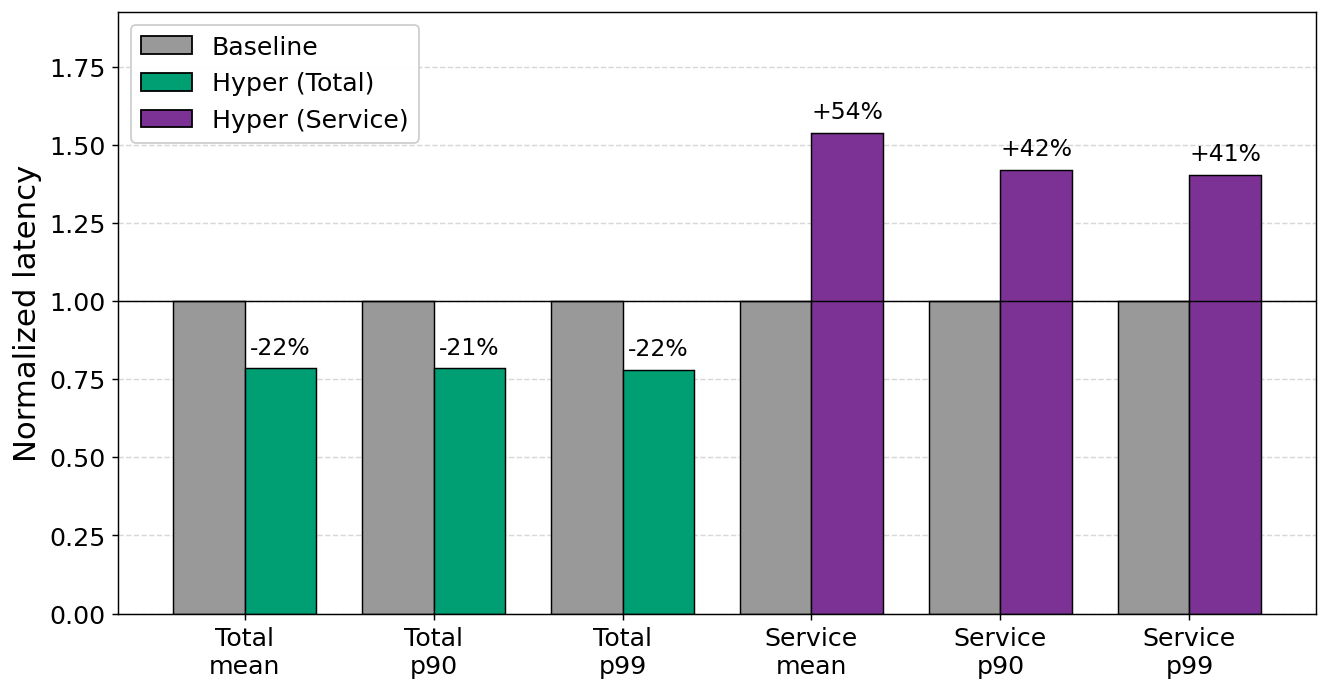
\includegraphics[width=\columnwidth]{hyper_v3_vs_baseline.png}
\caption{Normalized latency: \textsc{HyperAgent} vs.\ baseline. Total latency (end-to-end) drops 22\%, while service latency (worker-internal) rises because the engine is always busy.}
\label{fig:hyper}
\end{figure}

\textbf{\textsc{HyperAgenting} delivers a 22\% wall-time reduction and 28\% throughput improvement} (Table~\ref{tab:results}, Figure~\ref{fig:hyper}). Engine utilization jumps from 80\% to 98\%, confirming that partner switching fills tool-call idle windows. Mean latency drops from 46.3s to 36.3s because tasks complete faster when the engine is never idle.

\textbf{Engine queue time increases by two orders of magnitude, which is expected and healthy.} In baseline mode, the engine is mostly idle between tool calls, so requests face near-zero queueing. In \textsc{HyperAgent} mode, the engine always has work queued (the other partner), so individual requests wait longer. This cost is more than offset by eliminating idle GPU time.

\textbf{KV utilization stays below 1\% because the 7B model produces small caches relative to 80\,GB HBM.} At 72B scale, where one session at 2K tokens consumes 5\,GB, HBM pressure would be substantial and the tiering benefit proportionally larger. Our contribution is the scheduling mechanism and the proof that cooperative partner switching works.

\begin{figure}[t]
\centering
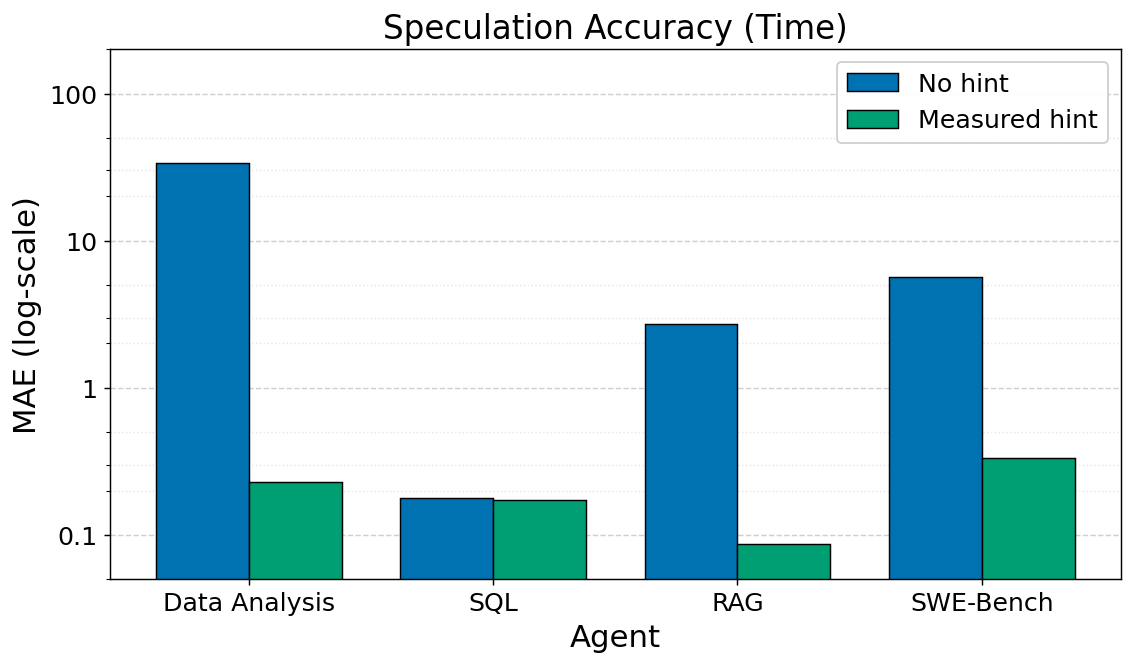
\includegraphics[width=\columnwidth]{speculation_time_mae.png}
\caption{Speculation accuracy (MAE in seconds, log scale). With measured hints from prior tool calls, duration prediction error drops by over an order of magnitude for Data Analysis and RAG agents.}
\label{fig:speculation}
\end{figure}

\textbf{Speculation accuracy.} We measured the model's ability to predict tool-call duration from conversation context (Figure~\ref{fig:speculation}). Without hints, Data Analysis agents have the highest prediction error (MAE $\approx$34s) due to their wide duration spread. With measured hints from prior calls in the same session, MAE drops to under 0.3s for all agent types except \textsc{Swe-Bench}. SQL agents show the smallest gap between hint and no-hint because their tool calls are consistently short. These coarse predictions suffice for tier selection (DRAM vs.\ SSD vs.\ keep in HBM).

\section{Reflection}
\label{sec:reflection}

\subsection{What Worked}

\textbf{The agent infrastructure is robust and generalizes well.} All four agent types run reliably on real benchmarks, produce correct answers, and generate clean traces. The trace format and visualizer proved valuable beyond their original purpose: per-tool-call KV snapshots from the real block manager validated analytical models against measured data, and the Gantt-style timeline view made it easy to spot scheduling pathologies by visual inspection.

\textbf{Early scheduling results are promising.} \textsc{HyperAgenting} was simple to implement (under 300 lines of Python) because it delegates all KV management to vLLM's existing preemption path. The 22\% wall-time improvement and 98\% engine utilization on a first prototype suggest that agent-aware scheduling has substantial room to grow with more aggressive policies and larger models.

\subsection{What Did Not Work}

\textbf{Custom eviction policies hit vLLM's abstraction boundary.} We originally planned to implement tiering decisions inside \texttt{AgentAwareBlockManager}, using predicted idle durations to choose between DRAM and SSD tiers. This requires hooking deeper into vLLM's scheduler than the block manager API permits: swap-in and swap-out decisions are made by the scheduler, not the block manager. Several side effects of vLLM's internal scheduling (e.g., how preemption interacts with prefix caching, how the priority scheduler handles concurrent requests) require deeper understanding of vLLM internals than our current instrumentation provides. We chose \textsc{HyperAgenting} as an alternative that achieves the same effect through a higher-level mechanism.

\textbf{Disk-based tiering is not yet implemented.} All current experiments use CPU swap (DRAM) only. SSD-based offloading requires either modifying vLLM's swap path to write to NVMe instead of host memory, or implementing a custom offload manager outside vLLM. This is the most important missing piece for the full three-tier vision.

\subsection{Next Steps}

\textbf{Focus on workloads where prefetching and offloading have the highest payoff.} The most promising use cases are agents with long prefills and short decodes. Our data shows prefill throughput is roughly 100$\times$ slower than decode in tokens per second; a session with 20K prefill tokens and 400 decode tokens spends most of its GPU time on prefill. Offloading that session's KV-cache during a tool call and prefetching it back saves recomputing those 20K tokens from scratch, a cost that dwarfs the transfer overhead. Future work should prioritize these high-prefill, low-decode workloads.

\textbf{Scale \textsc{HyperAgenting} beyond two partners.} The current design pairs exactly two tasks per worker. A fully stateful scheduler should manage an arbitrary number of concurrent tasks, proceeding aggressively on whichever task has the highest priority at each moment. This requires deeper integration with vLLM's scheduler to support fine-grained preemption across many sequences.

\textbf{Test across hardware and model configurations.} Our results are from a single H100 with a 7B model. Different GPU generations (A100, L40, consumer GPUs) have different HBM capacities and PCIe bandwidths, changing the tiering thresholds. Different model sizes (72B, 405B) change the KV-cache footprint per token. A systematic sweep across these configurations would quantify where tiering provides the most benefit.

\subsection{Milestones}

\textbf{We achieved progress between the 100\% and 125\% project goals.} Trace-driven workload characterization (75\% goal) is complete. Prediction-aware scheduling via \textsc{HyperAgenting} that shifts the Pareto frontier (100\% goal) is demonstrated. Batched concurrent agents with KV-swap preemption (125\% stretch goal) is partially achieved: the cooperative scheduling works, but disk-based tiering and multi-partner scaling remain as future work.

\section{AI Usage Report}

\subsection{How I Used AI}

\textbf{AI was the primary coding tool throughout this project; every module was either drafted or substantially edited by an LLM.} I used Claude Code (Anthropic's CLI agent, backed by Claude Opus and Sonnet) as my main development partner. GitHub Copilot handled routine autocompletion inside VS Code. The project itself is about serving LLM agents, so the tool and the subject overlapped in ways that were both productive and occasionally disorienting.

Claude Code wrote the first drafts of the ReAct agent loop, the trace collector, the vLLM engine wrapper, the \textsc{HyperAgent} scheduler, and all benchmark harnesses. My role was architecture decisions, prompt engineering for the coding agent, reviewing generated code, debugging runtime failures, and designing experiments. A typical cycle looked like: I described what I wanted in natural language, Claude Code produced a working module, I ran it, hit an error (usually a vLLM API mismatch or an async race condition), pasted the traceback back, and Claude Code fixed it. For the \textsc{HyperAgent} scheduler, this loop took three iterations to get the partner state machine right. For the tool-call parser, it took over ten iterations because Qwen's output format kept surprising us with edge cases.

\subsection{What I Learned}

\textbf{AI can make dangerous assumptions, and I learned to read every response carefully.} Early in the project, I trusted Claude Code's output after a quick glance. This led to two serious bugs that looked correct in code review but were only caught by examining traces:

\begin{enumerate}[nosep,leftmargin=*]
\item \textbf{The \textsc{Swe-Bench} agent was modifying test files instead of source files.} It appeared to ``fix'' bugs by weakening assertions. The code passed all checks Claude Code suggested, and Claude Code itself found no issue when asked to review.
\item \textbf{Brave Search API rate limits were being hit silently.} The API returned empty results instead of an error, so the RAG agent concluded there was no information available and gave a plausible-sounding but wrong answer. Again, the code looked correct; only the trace showed zero search results on queries that should have returned many.
\end{enumerate}

After these incidents, I added a rule to my Claude Code configuration file (CLAUDE.md): ``Always ask questions if something is unclear. We are doing research and it is a big task. Don't worry to ask questions.'' This forced the AI to surface uncertainty rather than making silent assumptions, and it measurably reduced the rate of subtle bugs in subsequent modules.

\textbf{LLM coding agents excel at boilerplate but struggle with stateful concurrency.} The entire trace infrastructure (tracer.py, about 200 lines) was generated in one shot and needed only minor edits. But the async engine integration required me to read vLLM source code myself and explain the internal scheduler API to Claude Code before it could produce correct wrappers. Prompt specificity matters enormously: vague requests like ``make the engine async'' produced broken code, while precise requests like ``wrap AsyncLLMEngine.generate as an async generator, yield RequestOutput, and extract metrics.first\_token\_time'' worked on the first try.

\subsection{What I Did Not Expect}

The biggest surprise was how much time I spent debugging AI-generated code that looked correct but had subtle concurrency bugs. The \textsc{HyperAgent} worker originally awaited both partners' futures with \texttt{asyncio.gather}, which deadlocked when both partners needed the engine simultaneously. Claude Code confidently produced this code and confidently defended it when I questioned it. I had to draw the state machine on paper, identify the deadlock, and then tell Claude Code exactly what to replace it with (\texttt{asyncio.wait} with \texttt{FIRST\_COMPLETED}). The lesson is that AI coding agents are not yet reliable for concurrent control flow; they generate plausible-looking code that passes superficial review but fails under contention.

\subsection{Maintaining Context Across Sessions with next\_session.md}

\textbf{One practice that proved essential was maintaining a \texttt{next\_session.md} file at the project root.} Claude Code sessions have limited context windows, and this project ran across many sessions over several weeks. At the end of each session, I wrote (or had Claude Code write) a structured handoff document that the next session could read to get up to speed immediately. The file included:

\begin{itemize}[nosep,leftmargin=*]
\item \textbf{What was done this session.} Concrete deliverables: which modules were written, which experiments were submitted, which bugs were fixed.
\item \textbf{What is pending.} SLURM job IDs, output paths, expected results. For example, after submitting the A100 sweep (N=8 through N=256), the file listed all six job IDs, the exact output paths for \texttt{batch\_summary.json} and \texttt{engine\_trace.json}, and shell commands to check job status.
\item \textbf{A morning checklist.} Step-by-step instructions for the next session: verify jobs finished, read sweep results, identify the breakpoint where KV pool saturates, decide next experiment. This was not prose; it was copy-pasteable shell commands with \texttt{python3 -c} one-liners to parse JSON results.
\item \textbf{Decision tree for next steps.} ``If the breakpoint isn't reached at N=256, shrink gpu\_memory\_utilization. If tasks are too short, raise the tool-call cap.'' This forced me to think ahead while the context was fresh, rather than re-derive the reasoning next session.
\item \textbf{Carryover bugs.} Open issues that were not fixed this session but should not be forgotten: \texttt{gold\_answer} dropped from traces, \texttt{python\_exec} pandas path bug, dead code in \texttt{agent/loop.py}.
\item \textbf{File references.} Exact file paths and line numbers for code that was changed or is relevant. This saved the next session from searching the codebase.
\end{itemize}

This file turned out to be the single most valuable artifact for working with AI across sessions. Without it, each new session started with Claude Code asking what the project does and what was last done. With it, I could paste \texttt{next\_session.md} into the context and the AI was immediately productive. The overhead of writing it (5 minutes at the end of a session) saved 15--20 minutes of re-orientation at the start of the next one.

I also maintained a \texttt{CLAUDE.md} configuration file with persistent rules for the AI: coding style, communication preferences, what not to touch, and explicit instructions like ``solve things step by step'' and ``never do what you have not been asked to do.'' This file was automatically loaded by Claude Code at session start, so the AI's behavior was consistent across sessions without repeating instructions.

\subsection{Project-Specific AI Experiences}

\textbf{Benchmark curation was surprisingly effective with AI.} I gave Claude Code the benchmark APIs (HotpotQA, BrowseComp, GAIA) and asked it to build a curated pool of 512 tasks with balanced representation. It wrote \texttt{build\_sweep512.py} in one pass: loading from each source, deduplicating, stratifying by difficulty level, and serializing to JSON with a fixed random seed for reproducibility. This is exactly the kind of mechanical but fiddly task where AI saves real time.

\textbf{SLURM job scripting was another strength.} Claude Code generated the sweep submission scripts (\texttt{submit\_sweep.sh}, \texttt{run\_a100\_one\_n.sh}) that parameterized concurrency via environment variables, set up the correct conda environment, and handled output directory creation. I ran these on the Harvard SEAS cluster without modification.

\textbf{vLLM internals were the hardest domain for AI.} vLLM's codebase is large, fast-moving, and full of version-specific APIs. Claude Code frequently guessed wrong about which class to subclass or which method signature to use, because its training data contained multiple vLLM versions. I had to read vLLM source myself, identify the correct API for version 0.7.3, and paste the relevant source files into Claude Code's context before it could produce working code. The MIG workaround is a good example: Claude Code had no idea that \texttt{CUDA\_VISIBLE\_DEVICES} could contain a MIG UUID string, because this is a niche deployment detail. I found the crash, read the vLLM platform detection code, and told Claude Code exactly what to patch.

\footnotesize
\bibliographystyle{plain}
\begin{thebibliography}{10}

\bibitem{kwon2023vllm}
W.~Kwon et al., ``Efficient memory management for large language model serving with PagedAttention,'' \emph{SOSP}, 2023.

\bibitem{yao2023react}
S.~Yao et al., ``ReAct: Synergizing reasoning and acting in language models,'' \emph{ICLR}, 2023.

\bibitem{continuum2024}
Hanchen Li et al., ``Continuum: Serving AI agents with scalable long-context efficiency,'' \emph{arXiv:2511.02230}, 2024.

\bibitem{yang2024swebench}
J.~Yang et al., ``SWE-bench: Can language models resolve real-world GitHub issues?'' \emph{ICLR}, 2024.

\bibitem{yang2018hotpotqa}
Z.~Yang et al., ``HotpotQA: A dataset for diverse, explainable multi-hop question answering,'' \emph{EMNLP}, 2018.

\bibitem{wei2025browsecomp}
J.~Wei et al., ``BrowseComp: A simple challenge for browsing agents,'' \emph{OpenAI Research}, 2025.

\bibitem{mialon2023gaia}
G.~Mialon et al., ``GAIA: A benchmark for general AI assistants,'' \emph{arXiv:2311.12983}, 2023.

\bibitem{li2024lmcache}
G.~Li et al., ``LMCache: A knowledge delivery network for efficient LLM inference,'' \emph{arXiv:2510.09665}, 2024.

\bibitem{qin2025mooncake}
R.~Qin et al., ``Mooncake: Trading more storage for less computation,'' \emph{FAST}, 2025.

\bibitem{sheng2023flexgen}
Y.~Sheng et al., ``FlexGen: High-throughput generative inference of large language model serving with a single GPU,'' \emph{ICML}, 2023.

\end{thebibliography}

\end{document}
